\documentclass[border=5pt]{standalone}
\usepackage{mathptmx}
\usepackage[T1]{fontenc}
\usepackage{tikz}
\usetikzlibrary{shapes.geometric,shapes.misc,arrows.meta,positioning,calc,fit,shadows.blur}
\usepackage{xcolor}

\definecolor{diagLaw}{HTML}{1D6FE0}
\definecolor{diagPlan}{HTML}{E63946}
\definecolor{diagEnv}{HTML}{12A150}
\definecolor{diagLatent}{HTML}{7C3AED}
\definecolor{diagProbe}{HTML}{E8890C}
\definecolor{gapblue}{HTML}{00B4D8}
\definecolor{gapred}{HTML}{C2185B}
\definecolor{inkmute}{HTML}{6B7280}

\begin{document}
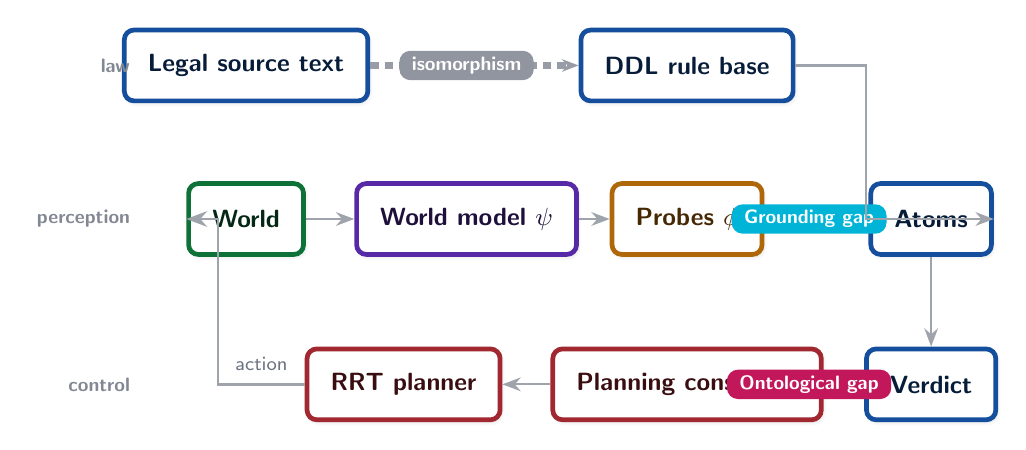
\begin{tikzpicture}[
    >=Stealth,
    font=\sffamily\small,
    % Flat fill + a HEAVY tinted border carries the node identity; the blur shadow is barely there
    % (opacity 0.12) so it lifts the card off the page without reading as a 2005 gradient.
    card/.style={draw, line width=1.7pt, rounded corners=3.5pt, align=center,
                 minimum height=9mm, inner xsep=3mm, font=\sffamily\small\bfseries,
                 blur shadow={shadow blur steps=8, shadow xshift=0.6pt, shadow yshift=-0.9pt,
                              shadow opacity=12, shadow blur radius=1.4pt}},
    env/.style ={card, fill=white, draw=diagEnv!70!black,    text=diagEnv!25!black},
    lat/.style ={card, fill=white, draw=diagLatent!70!black, text=diagLatent!25!black},
    prb/.style ={card, fill=white, draw=diagProbe!75!black,  text=diagProbe!30!black},
    law/.style ={card, fill=white, draw=diagLaw!70!black,    text=diagLaw!25!black},
    pln/.style ={card, fill=white, draw=diagPlan!70!black,   text=diagPlan!25!black},
    % Ordinary dataflow is deliberately recessive: thin, grey. The gaps must win the page.
    flow/.style={->, line width=0.8pt, draw=inkmute!65},
    % THE MOTIF. The two gaps are the conceptual punchline, so they are the thickest marks here.
    gap/.style={line width=2.4pt, dash pattern=on 5.5pt off 3pt, -{Stealth[length=6pt]}},
    % Solid colour capsule, white text, sitting ON the line it names.
    caps/.style={fill=#1, text=white, rounded corners=4pt, inner xsep=4.5pt, inner ysep=2.2pt,
                 font=\sffamily\scriptsize\bfseries},
    bandlab/.style={font=\sffamily\scriptsize\bfseries, text=inkmute!85, anchor=east},
]

%================= ROW 1 : the legal source, and the CLASSICAL isomorphism =================%
\node[law] (statute) at (0,2.55)   {Legal source text};
\node[law] (rules)   at (5.6,2.55) {DDL rule base};
\draw[gap, draw=inkmute!70, dash pattern=on 3pt off 2.2pt] (statute) -- (rules);
\node[caps=inkmute!75] at ($(statute)!0.5!(rules)$) {isomorphism};

%================= ROW 2 : world -> atoms  (the GROUNDING gap) =================%
\node[env] (world)  at (0,0.6)   {World};
\node[lat] (wm)     at (2.8,0.6) {World model $\psi$};
\node[prb] (probes) at (5.6,0.6) {Probes $\phi$};
\node[law] (atoms)  at (8.7,0.6) {Atoms};
\draw[flow] (world) -- (wm);
\draw[flow] (wm) -- (probes);
\draw[gap, draw=gapblue] (probes) -- (atoms);
\node[caps=gapblue] at ($(probes)!0.5!(atoms)$) {Grounding gap};

%================= ROW 3 : verdict -> constraint  (the ONTOLOGICAL gap) =================%
\node[law] (verdict) at (8.7,-1.5) {Verdict};
\node[pln] (cons)    at (5.6,-1.5) {Planning constraint};
\node[pln] (planner) at (2.0,-1.5) {RRT planner};
\draw[flow] (rules.east) -- ++(0.9,0) |- (atoms.east);
\draw[flow] (atoms) -- (verdict);
\draw[gap, draw=gapred] (verdict) -- (cons);
\node[caps=gapred] at ($(verdict)!0.5!(cons)$) {Ontological gap};
\draw[flow] (cons) -- (planner);

%================= the closed loop, made explicit =================%
\draw[flow, line width=1.0pt] (planner.west) -- ++(-1.1,0)
      node[midway, above=1pt, font=\sffamily\scriptsize, text=inkmute] {action} |- (world.west);

%================= band labels =================%
\node[bandlab] at (-1.35,2.55) {\textsc{law}};
\node[bandlab] at (-1.35,0.6)  {\textsc{perception}};
\node[bandlab] at (-1.35,-1.5) {\textsc{control}};

\end{tikzpicture}
\end{document}
